\documentclass{standalone}
\usepackage{tikz}
\usepackage{mathrsfs}
\usetikzlibrary{positioning, shapes.geometric, arrows}
\usepackage[T1]{fontenc}
\renewcommand*\familydefault{\ttdefault} %% Only if the base font of the document is to be typewriter style
\begin{document}
	 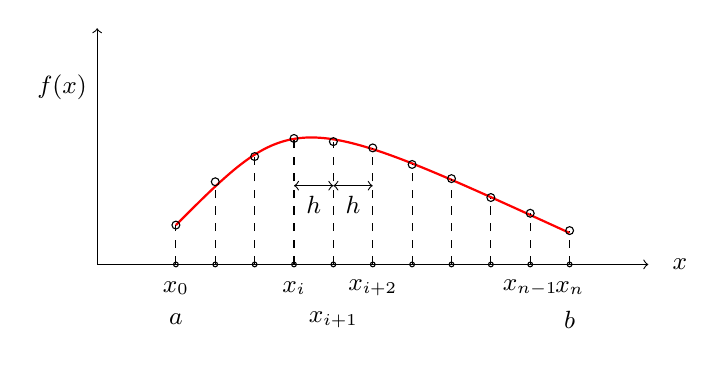
\begin{tikzpicture}[font=\small]
		\draw [->] (0,0) -- node [near end, left]{$f(x)$} (0,3);
		\draw [->] (0,0) -- (7,0);
		\draw (7.4,0) node {$x$};
		\draw [red, thick] (1,0.5) .. controls(2.5,2) .. (6,0.4);
		\foreach \x in {1,1.5,...,6} \draw (\x,0) circle (0.03cm);
		\draw (1,-0.3) node {$x_{0}$};
		\draw (1,-0.7) node {$a$};
		%\draw (1.5,-0.3) node {$x_{1}$};
		%\draw (2,-0.3) node {$x_{2}$};
		\draw (2.5,-0.3) node {$x_{i}$};
		\draw (3,-0.7) node {$x_{i + 1}$};
		\draw (3.5,-0.3) node {$x_{i + 2}$};
		\draw (5.5,-0.3) node {$x_{n - 1}$};
		\draw (6,-0.3) node {$x_{n}$};
		\draw (6,-0.7) node {$b$};
		\draw [dashed] (1,0) -- (1,0.5);
		\draw [dashed] (1.5,0) -- (1.5,1.05);
		\draw [dashed] (2,0) -- (2,1.37);
		\draw [dashed] (2.5,0) -- (2.5,1.6);
		\draw [dashed] (3,0) -- (3,1.56);
		\draw [dashed] (3.5,0) -- (3.5,1.48);
		\draw [dashed] (4,0) -- (4,1.27);
		\draw [dashed] (4.5,0) -- (4.5,1.09);
		\draw [dashed] (5,0) -- (5,0.85);
		\draw [dashed] (5.5,0) -- (5.5,0.65);
		\draw [dashed] (6,0) -- (6,0.43);
		\draw (1,0.5) circle (0.05);
		\draw (1.5,1.05) circle (0.05);
		\draw (2,1.37) circle (0.05);
		\draw (2.5,1.6) circle (0.05);
		\draw (3,1.56) circle (0.05);
		\draw (3.5,1.48) circle (0.05);
		\draw (4,1.27) circle (0.05);
		\draw (4.5,1.09) circle (0.05);
		\draw (5,0.85) circle (0.05);
		\draw (5.5,0.65) circle (0.05);
		\draw (6,0.43) circle (0.05);
		\draw [<->] (2.5,1) -- node [midway, below] {$h$} (3,1);
		\draw [<->] (3,1) -- node [midway, below] {$h$} (3.5,1);
\end{tikzpicture}
\end{document}